% ============================================================================
% 甄嬛传·千声千面 —— AI 角色语音对话系统
% 终期论文
% ============================================================================
% 成员A: 李思婷 2023212061 — 数据处理与CosyVoice模型训练
% 成员B: 张笑   2023212062 — GPT-SoVITS微调与ASR+LLM对话模块
% 成员C: 黄艺平 2023212179 — 前端设计与系统集成
% ============================================================================

\documentclass[12pt,a4paper]{article}

% ── 中文支持 ──────────────────────────────────────────────────────────────
\usepackage[UTF8,fontset=none]{ctex}
\setCJKmainfont{SimSun}[AutoFakeBold=2.5,AutoFakeSlant=0.2]
\setCJKsansfont{SimHei}[AutoFakeBold=2.5]
\setCJKmonofont{KaiTi}
\newCJKfontfamily\heiti{SimHei}[AutoFakeBold=2.5]
\setmainfont{Times New Roman}

% ── 页面布局 ──────────────────────────────────────────────────────────────
\usepackage[left=2.5cm, right=2.5cm, top=2.5cm, bottom=2.5cm]{geometry}
\usepackage{setspace}
\onehalfspacing
\setlength{\hfuzz}{25pt}
\hbadness=10000

% ── 图表与代码 ────────────────────────────────────────────────────────────
\usepackage{graphicx}
\usepackage{float}
\usepackage{booktabs}
\usepackage{longtable}
\usepackage{multirow}
\usepackage{array}
\usepackage{tabularx}
\usepackage{caption}
\usepackage{subcaption}
\usepackage{listings}
\usepackage[table]{xcolor}

% ── 代码样式 ──────────────────────────────────────────────────────────────
\lstset{
    basicstyle=\small\ttfamily,
    breaklines=true,
    frame=single,
    backgroundcolor=\color{gray!5},
    rulecolor=\color{gray!40},
    numbers=left,
    numberstyle=\tiny\color{gray},
    keywordstyle=\color{blue!70},
    commentstyle=\color{green!50!black},
    stringstyle=\color{red!60},
    showstringspaces=false,
    tabsize=4
}

% ── 链接与引用 ────────────────────────────────────────────────────────────
\usepackage[colorlinks=true,
            linkcolor=blue,
            citecolor=blue,
            urlcolor=blue]{hyperref}

% ── 数学与符号 ────────────────────────────────────────────────────────────
\usepackage{amsmath,amssymb}
\usepackage{enumitem}

% ── TikZ 流程图 ────────────────────────────────────────────────────────────
\usepackage{tikz}
\usetikzlibrary{
    shapes.geometric,
    arrows.meta,
    positioning,
    fit,
    backgrounds,
    calc
}
% 成员C专属配色（红色系）
\definecolor{Clight}{RGB}{253, 236, 234}
\definecolor{Cmid}{RGB}{192, 57, 43}
\definecolor{Cdark}{RGB}{145, 35, 28}
\definecolor{Cgray}{RGB}{253, 248, 247}
% 成员C流程图样式
\tikzset{
    cproc/.style={
        rectangle, rounded corners=6pt, draw=Cmid, line width=1.0pt,
        fill=white, text=black, minimum width=2.6cm, minimum height=0.9cm,
        align=center, font=\footnotesize\sffamily, inner sep=6pt
    },
    cterm/.style={
        rectangle, rounded corners=8pt, draw=Cdark, line width=1.2pt,
        fill=Cmid, text=white, minimum width=2.6cm, minimum height=0.95cm,
        align=center, font=\footnotesize\bfseries\sffamily, inner sep=6pt
    },
    carr/.style={-{Stealth[length=7pt, width=5pt]}, line width=0.9pt, Cdark},
}

% ── 页眉页脚 ──────────────────────────────────────────────────────────────
\usepackage{fancyhdr}
\setlength{\headheight}{14.5pt}
\pagestyle{fancy}
\fancyhf{}
\fancyhead[L]{甄嬛传·千声千面 —— AI 角色语音对话系统}
\fancyhead[R]{终期论文}
\fancyfoot[C]{\thepage}
\renewcommand{\headrulewidth}{0.4pt}


% ══════════════════════════════════════════════════════════════════════════
\begin{document}

% ── 封面页 ────────────────────────────────────────────────────────────────
\begin{titlepage}
\thispagestyle{empty}

\vspace*{1.5cm}

\begin{center}

\includegraphics[width=0.55\textwidth]{北邮校名校徽编排 横版中英文.png}
\end{center}

\vspace{1.8cm}

\begin{center}
{\Large\heiti ——\; 语音信息处理大作业 \;\textbullet\; 终期论文 \;——}
\end{center}

\vspace{2.5cm}

\begin{center}
{\fontsize{28pt}{36pt}\selectfont\heiti
甄嬛传·千声千面\\[10pt]
AI 角色语音对话系统}
\end{center}

\vspace{3.5cm}

\begin{center}
{\large
\renewcommand{\arraystretch}{1.6}
\begin{tabular}{rll}
    \textbf{成员A} & \textbf{李思婷} & 2023212061 \\
    \textbf{成员B} & \textbf{张笑}   & 2023212062 \\
    \textbf{成员C} & \textbf{黄艺平} & 2023212179 \\
\end{tabular}
}
\end{center}

\vfill

\begin{center}
{\large 2026 年 6 月}
\end{center}

\vspace{1cm}

\end{titlepage}

% ── 摘要 ──────────────────────────────────────────────────────────────────
\newpage
\pagenumbering{Roman}

\begin{center}
{\LARGE\heiti 摘\quad 要}
\end{center}
\vspace{0.5cm}

本文介绍了一个面向电视剧《甄嬛传》的 AI 角色语音对话系统------\,\textbf{甄嬛传\,\textperiodcentered\,千声千面}。该系统从 76 集原剧音频中自主构建了包含 14 个角色、13,605 段语音片段（总时长约 16.7 小时）的高质量中文语音数据集，并基于 CosyVoice3-0.5B（Zero-shot 语音克隆）和 GPT-SoVITS（微调语音合成）双引擎实现了多角色语音克隆与情感语音合成。系统结合大语言模型（LLM）实现角色性格建模与对话生成，支持单人智能对话与双人即兴对戏两种交互模式，并通过 SSE 流式传输与 Web Audio API 实现了低延迟的语音播放体验。实验表明，CosyVoice3 Zero-shot 方案在音色还原度和自然度上显著优于微调方案，创新性的\textbf{情绪 Speaker}方案有效解决了情绪控制与音色保真之间的矛盾。

\vspace{0.8cm}
\noindent\textbf{关键词：}语音克隆；语音合成；CosyVoice；GPT-SoVITS；大语言模型；说话人识别；情感语音合成

% ── 目录 ──────────────────────────────────────────────────────────────────
\newpage
\tableofcontents
\newpage
\pagenumbering{arabic}
\setcounter{page}{1}

% ══════════════════════════════════════════════════════════════════════════
\section{选题背景}
\label{sec:background}

\subsection{研究背景}

语音合成（Text-to-Speech, TTS）与语音克隆（Voice Cloning）技术在近年来取得了飞速发展。以 VALL-E、CosyVoice、GPT-SoVITS 等为代表的新一代语音合成模型，凭借强大的零样本（Zero-shot）学习能力和细粒度的韵律控制，使得高质量的个性化语音合成成为可能。与此同时，大语言模型（LLM）在自然语言理解与生成方面的突破，为构建具有角色个性的智能对话系统提供了新思路。

影视IP的语音交互应用是上述技术的典型落地场景。《甄嬛传》作为中国最具影响力的古装电视剧之一，拥有大量经典角色和丰富的台词素材，其角色声音具有高辨识度和情感表现力，是语音克隆技术的理想实验对象。然而，将语音克隆技术应用于多角色场景面临若干挑战：首先，从原始音频中提取并标注多角色数据需要完整的音频处理流水线；其次，多角色联合训练容易因数据不均衡导致过拟合；最后，在保持音色保真的同时实现情绪控制是一个尚未充分解决的问题。

\subsection{课程要求}

本项目为\textbf{语音信息处理}课程大作业，要求涵盖语音合成、语音克隆、说话人识别、情感识别等核心技术，具备完整的算法实现、自主构建数据集的能力，并展示创新应用场景。

% ══════════════════════════════════════════════════════════════════════════
\section{实验目标}
\label{sec:objectives}

本项目旨在构建一个面向《甄嬛传》的 AI 角色语音对话系统，实现以下核心目标：

\begin{enumerate}[leftmargin=*]
    \item \textbf{自主构建多角色语音数据集}：从 76 集原剧音频出发，通过人声分离、语音识别、声纹聚类与人工标注，构建包含 14 个角色的高质量中文语音数据集。
    \item \textbf{多角色语音克隆与合成}：基于 CosyVoice3-0.5B（Zero-shot）和 GPT-SoVITS（微调）双引擎实现角色声音的高保真复现，支持用户实时对比两种引擎的合成效果。
    \item \textbf{情感语音合成}：实现喜悦、愤怒、悲伤、平静四种情绪的语音合成，在不损失音色保真度的前提下自然表达角色情感。
    \item \textbf{角色智能对话}：结合 LLM 实现角色性格建模，支持\textbf{现代来客}和\textbf{宫廷中人}两种身份的单人对话，以及双角色自动即兴对戏。
    \item \textbf{完整系统集成}：构建包含 React 前端、FastAPI 后端中间层、云端 TTS/ASR/LLM 服务的完整系统，实现流式语音播放和实时交互。
\end{enumerate}

% ══════════════════════════════════════════════════════════════════════════
\section{方法流程}
\label{sec:methods}

本节详细介绍系统各模块的技术方案与实现细节。

% TODO: 后续可插入系统整体架构图
% \begin{figure}[H]
% \centering
% \includegraphics[width=0.95\textwidth]{figures/system_architecture.png}
% \caption{系统整体架构图}
% \label{fig:system-arch}
% \end{figure}

% ── 3.1 数据集构建 ────────────────────────────────────────────────────────
\subsection{数据集构建}
\label{sec:data}

% [成员A负责撰写]
% 此部分介绍从76集原剧音频构建14角色语音数据集的完整流程，包括：
%
% 1. 数据来源与规模（76集MP3, 约80小时）
% 2. 数据处理Pipeline（五步流程）：
%    - Step 1: UVR5人声分离（mdx_extra_q模型，去除背景音乐与环境噪声）
%    - Step 2: FunASR VAD切分 + ASR转写（SeacoParaformer, 时间戳合并, 15685段）
%    - Step 3: 声纹提取与说话人聚类（eres2netv2 512维embedding + KMeans n=30）
%    - Step 4: 人工角色标注（关键词辅助系统 + 三轮迭代, 确认14角色）
%    - Step 5: 数据清洗与质量过滤（角色过滤→文本过滤→文本去重→音频质检）
% 3. 最终数据集统计（14角色, 13605段, 约16.7小时）
% 4. 数据分布分析（甄嬛占比最高约30%, 数据极度不均衡）
%
% 可配合Pipeline流程图和数据分布表

% ── 3.2 CosyVoice3 语音克隆 ──────────────────────────────────────────────
\subsection{CosyVoice3 语音克隆}
\label{sec:cosyvoice}

% [成员A负责撰写]
% 此部分介绍CosyVoice3-0.5B的微调实验与最终Zero-shot方案，包括：
%
% 1. CosyVoice3-0.5B 微调实验：
%    - 训练配置（RTX 4080 SUPER, lr=1e-5, batch 800 frames等）
%    - 训练过程记录（Epoch 0-5的loss和accuracy变化）
%    - 过拟合问题分析（Epoch 3开始CV Loss反转上升）
% 2. 从微调转向Zero-shot的决策分析：
%    - 微调 vs Zero-shot的对比（数据需求、训练时间、音色质量、可扩展性）
% 3. 14角色Zero-shot Speaker注册：
%    - 每角色精选1条高质量参考音频 + 台词文本
%    - add_zero_shot_spk 提取声纹特征 → spk2info.pt 持久化
% 4. 情绪Speaker创新方案：
%    - 情绪控制与音色保真的矛盾
%    - 从76集原剧手工筛选4主角×4情绪=107段真实情绪音频
%    - 注册为独立情绪Speaker（共30个Speaker: 14基础+16情绪）
%    - 推理时的情绪路由机制
%
% 建议配合微调loss曲线图和情绪Speaker注册统计表

% ── 3.3 GPT-SoVITS 微调 ──────────────────────────────────────────────────
\subsection{GPT-SoVITS 微调}
\label{sec:gptsovits}

% [成员B负责撰写]
% 此部分介绍GPT-SoVITS的微调训练流程与策略，包括：
%
% 1. 数据准备（转换为标准list格式, 按角色拆分train/dev）
% 2. 微调核心策略：
%    - 单角色独立微调（不混合训练, 降低音色混淆）
%    - 双版本并行（v4主版本 + v2ProPlus备选版本）
%    - LoRA微调（lora_rank=32, 降低过拟合风险）
%    - 批量自动化训练脚本
% 3. 训练流程（文本特征提取→HuBERT特征提取→Semantic Token提取→SoVITS训练→GPT训练）
% 4. 训练规模（14角色×2版本=28组独立权重）
% 5. 情绪参考音频路由设计
%
% 建议配合训练流程图和权重统计表

% ── 3.4 ASR + LLM 对话模块 ───────────────────────────────────────────────
\subsection{ASR + LLM 对话模块}
\label{sec:asr-llm}

% [成员B负责撰写]
% 此部分介绍语音识别和大语言模型对话生成模块，包括：
%
% 1. ASR语音识别：
%    - 模型选择（faster-whisper-small, 中文准确率与速度的平衡）
%    - 推理配置（VAD过滤、中文强约束、模型缓存）
%    - 前端交互策略（识别结果回填输入框, 用户确认后发送）
% 2. LLM单人对话Prompt设计：
%    - system_prompt + user_prompt 分层架构
%    - 一次生成展示文本+情绪标签+双TTS文本
%    - 现代来客 vs 宫廷中人身份感知对话
% 3. 双人即兴对话Prompt设计：
%    - 完整历史传递 + 双方角色人设独立注入
%    - 交替发言角色, 循环调用LLM
% 4. 双TTS文本策略：
%    - CosyVoice允许副语言token（[breath][laughter]等）
%    - GPT-SoVITS自动清洗为干净中文文本
%
% 建议配合Prompt示例和对话链路流程图

% ── 3.5 前端设计与系统集成 ───────────────────────────────────────────────
\subsection{前端设计与系统集成}
\label{sec:frontend}

本模块负责用户交互界面和系统各服务的集成调度，包括 React 前端 UI、yiping-backend 中间层，以及流式音频播放链路。

\subsubsection{整体架构}

系统采用前后端分离架构，前端 React 应用通过 yiping-backend 中间层统一调度云端各服务。整体架构如图~\ref{fig:system-arch}所示。

\begin{figure}[H]
\centering
\begin{tikzpicture}[node distance=1.4cm and 2.0cm, auto, scale=0.82, every node/.style={transform shape}]

    % ── 第一行：前端 ──────────────────────────────────────
    \node [cterm, minimum width=5.0cm]
        (frontend) {\textbf{React 前端} (\texttt{:5173}) \\ {\footnotesize Vite + React Router + Web Audio API}};

    % ── 第二行：中间层 ────────────────────────────────────
    \node [cproc, below=1.6cm of frontend, minimum width=5.0cm]
        (backend) {\textbf{yiping-backend} (\texttt{:8000}) \\ {\footnotesize FastAPI 中间层 \textperiodcentered{} 统一 API 网关}};

    % ── 第三行：三个云端服务（水平并排，加大间距避免标签重叠）
    \node [cproc, below=2.8cm of backend, xshift=-4.5cm, minimum width=3.4cm]
        (asr) {\textbf{ASR + LLM} (\texttt{:8001}) \\ {\footnotesize faster-whisper + LLM 对话}};
    \node [cproc, below=2.8cm of backend, minimum width=3.4cm]
        (gptsovits) {\textbf{GPT-SoVITS} (\texttt{:8002}) \\ {\footnotesize 14 角色微调权重}};
    \node [cproc, below=2.8cm of backend, xshift=4.5cm, minimum width=3.4cm]
        (cosyvoice) {\textbf{CosyVoice3} (\texttt{:8003}) \\ {\footnotesize 30 Speaker Zero-shot}};

    % ── 分组虚线框：AutoDL 云端 ──────────────────────────
    \begin{scope}[on background layer]
        \node [fit=(asr)(gptsovits)(cosyvoice),
               draw=Cdark, dashed, line width=0.7pt,
               rounded corners=10pt, inner sep=14pt]
               (cloud) {};
    \end{scope}
    \node [font=\footnotesize\bfseries\color{Cdark},
           fill=white, inner sep=2pt, anchor=south, yshift=2pt]
           at (cloud.north) {AutoDL 云端（RTX 4080 SUPER）};

    % ── 分组虚线框：本地 ──────────────────────────────────
    \begin{scope}[on background layer]
        \node [fit=(frontend)(backend),
               draw=Cmid, dashed, line width=0.7pt,
               rounded corners=10pt, inner sep=14pt]
               (local) {};
    \end{scope}
    \node [font=\footnotesize\bfseries\color{Cmid},
           fill=white, inner sep=2pt, anchor=south]
           at (local.north) {本地 Windows};

    % ── 箭头 ─────────────────────────────────────────────
    \draw [carr] (frontend) -- node[right, font=\scriptsize\color{Cdark}, xshift=2pt]{HTTP / SSE} (backend);
    \draw [carr] (backend) -- (asr);
    \draw [carr] (backend) -- (gptsovits);
    \draw [carr] (backend) -- (cosyvoice);

    % ── SSH 隧道标注（放在中间箭头左侧，避免与云端标签重叠）
    \node [font=\scriptsize\color{Cdark}, fill=white, inner sep=1pt,
           anchor=east, xshift=-6pt]
          at ($(backend.south)!0.45!(gptsovits.north)$) {SSH 隧道};

\end{tikzpicture}
\caption{系统整体架构图}
\label{fig:system-arch}
\end{figure}

yiping-backend 中间层对外提供统一的 RESTful API，各接口功能如表~\ref{tab:api}所示。

\begin{table}[H]
\centering
\caption{yiping-backend 接口列表}
\label{tab:api}
\begin{tabularx}{\textwidth}{p{4.2cm}p{3.2cm}X}
\toprule
\textbf{接口} & \textbf{调用服务} & \textbf{功能说明} \\
\midrule
\texttt{POST /asr}                & ASR (\texttt{:8001})       & 用户录音上传，返回识别文本 \\
\texttt{POST /chat}               & LLM (\texttt{:8001})       & 角色对话，返回回复文本 + 情绪标签 + 双 TTS 文本 \\
\texttt{POST /synthesize}         & GPT-SoVITS / CosyVoice   & 非流式语音合成，返回音频 URL \\
\texttt{POST /synthesize/stream}  & CosyVoice (\texttt{:8003}) & SSE 流式语音合成，逐块推送 base64 音频 \\
\texttt{POST /duet/start}         & LLM + TTS                 & 双人即兴对话，SSE 逐轮推流 \\
\texttt{POST /summary}            & LLM (\texttt{:8001})       & 对话总结，返回态度评价 + 古风总结语 \\
\bottomrule
\end{tabularx}
\end{table}

\subsubsection{前端技术栈与视觉设计}

前端采用 React + Vite 构建，使用纯 CSS（CSS Variables + Keyframes 动画）实现全部视觉效果，React Router 管理页面路由。视觉上确立了一套宫廷古风色彩体系，贯穿全部页面：深墨绿（\texttt{\#1a2a1a}）与深红褐（\texttt{\#2a1a1a}）为主色调，宫廷金（\texttt{\#c9a84c}）为强调色，标题使用 Ma Shan Zheng 毛笔体，正文使用宋体。所有视觉素材（14 张角色剧照、11 张场景背景图、1 首背景音乐《长相思》）均为自行搜集。

\subsubsection{页面架构}

系统包含四个核心页面，交互流程如图~\ref{fig:page-flow}所示。

\begin{figure}[H]
\centering
\begin{tikzpicture}[node distance=1.6cm and 1.8cm, auto, scale=0.82, every node/.style={transform shape}]

    % ── 四个页面节点 ──────────────────────────────────────
    \node [cterm, minimum width=3.6cm]
        (home) {\textbf{主页} \\ {\footnotesize Ken Burns 动效 + 背景音乐}};
    \node [cproc, below=1.6cm of home, minimum width=3.6cm]
        (select) {\textbf{角色选择页} \\ {\footnotesize 三种模式入口 + 14 角色卡片}};
    \node [cproc, below left=1.6cm and 2.0cm of select, minimum width=3.6cm]
        (chat) {\textbf{对话页} \\ {\footnotesize 语音/文字输入 + TTS 播放}};
    \node [cproc, below right=1.6cm and 2.0cm of select, minimum width=3.6cm]
        (duet) {\textbf{即兴对话页} \\ {\footnotesize 双角色自动对戏}};

    % ── 箭头 ─────────────────────────────────────────────
    \draw [carr] (home) -- (select);
    \draw [carr] (select) -- node[left, font=\scriptsize\color{Cdark}]{现代来客 / 宫廷中人} (chat);
    \draw [carr] (select) -- node[right, font=\scriptsize\color{Cdark}]{即兴对话} (duet);

\end{tikzpicture}
\caption{前端页面导航流程}
\label{fig:page-flow}
\end{figure}

\paragraph{主页（HomePage）}
全屏背景图叠加半透明遮罩，背景图使用 Ken Burns 缓动动效（\texttt{scale 1\(\to\)1.08}，15 秒循环）营造电影感。中央显示系统标题（毛笔体）与副标题，右下角提供背景音乐控制按钮。效果如图~\ref{fig:ui-home}所示。

\begin{figure}[H]
\centering
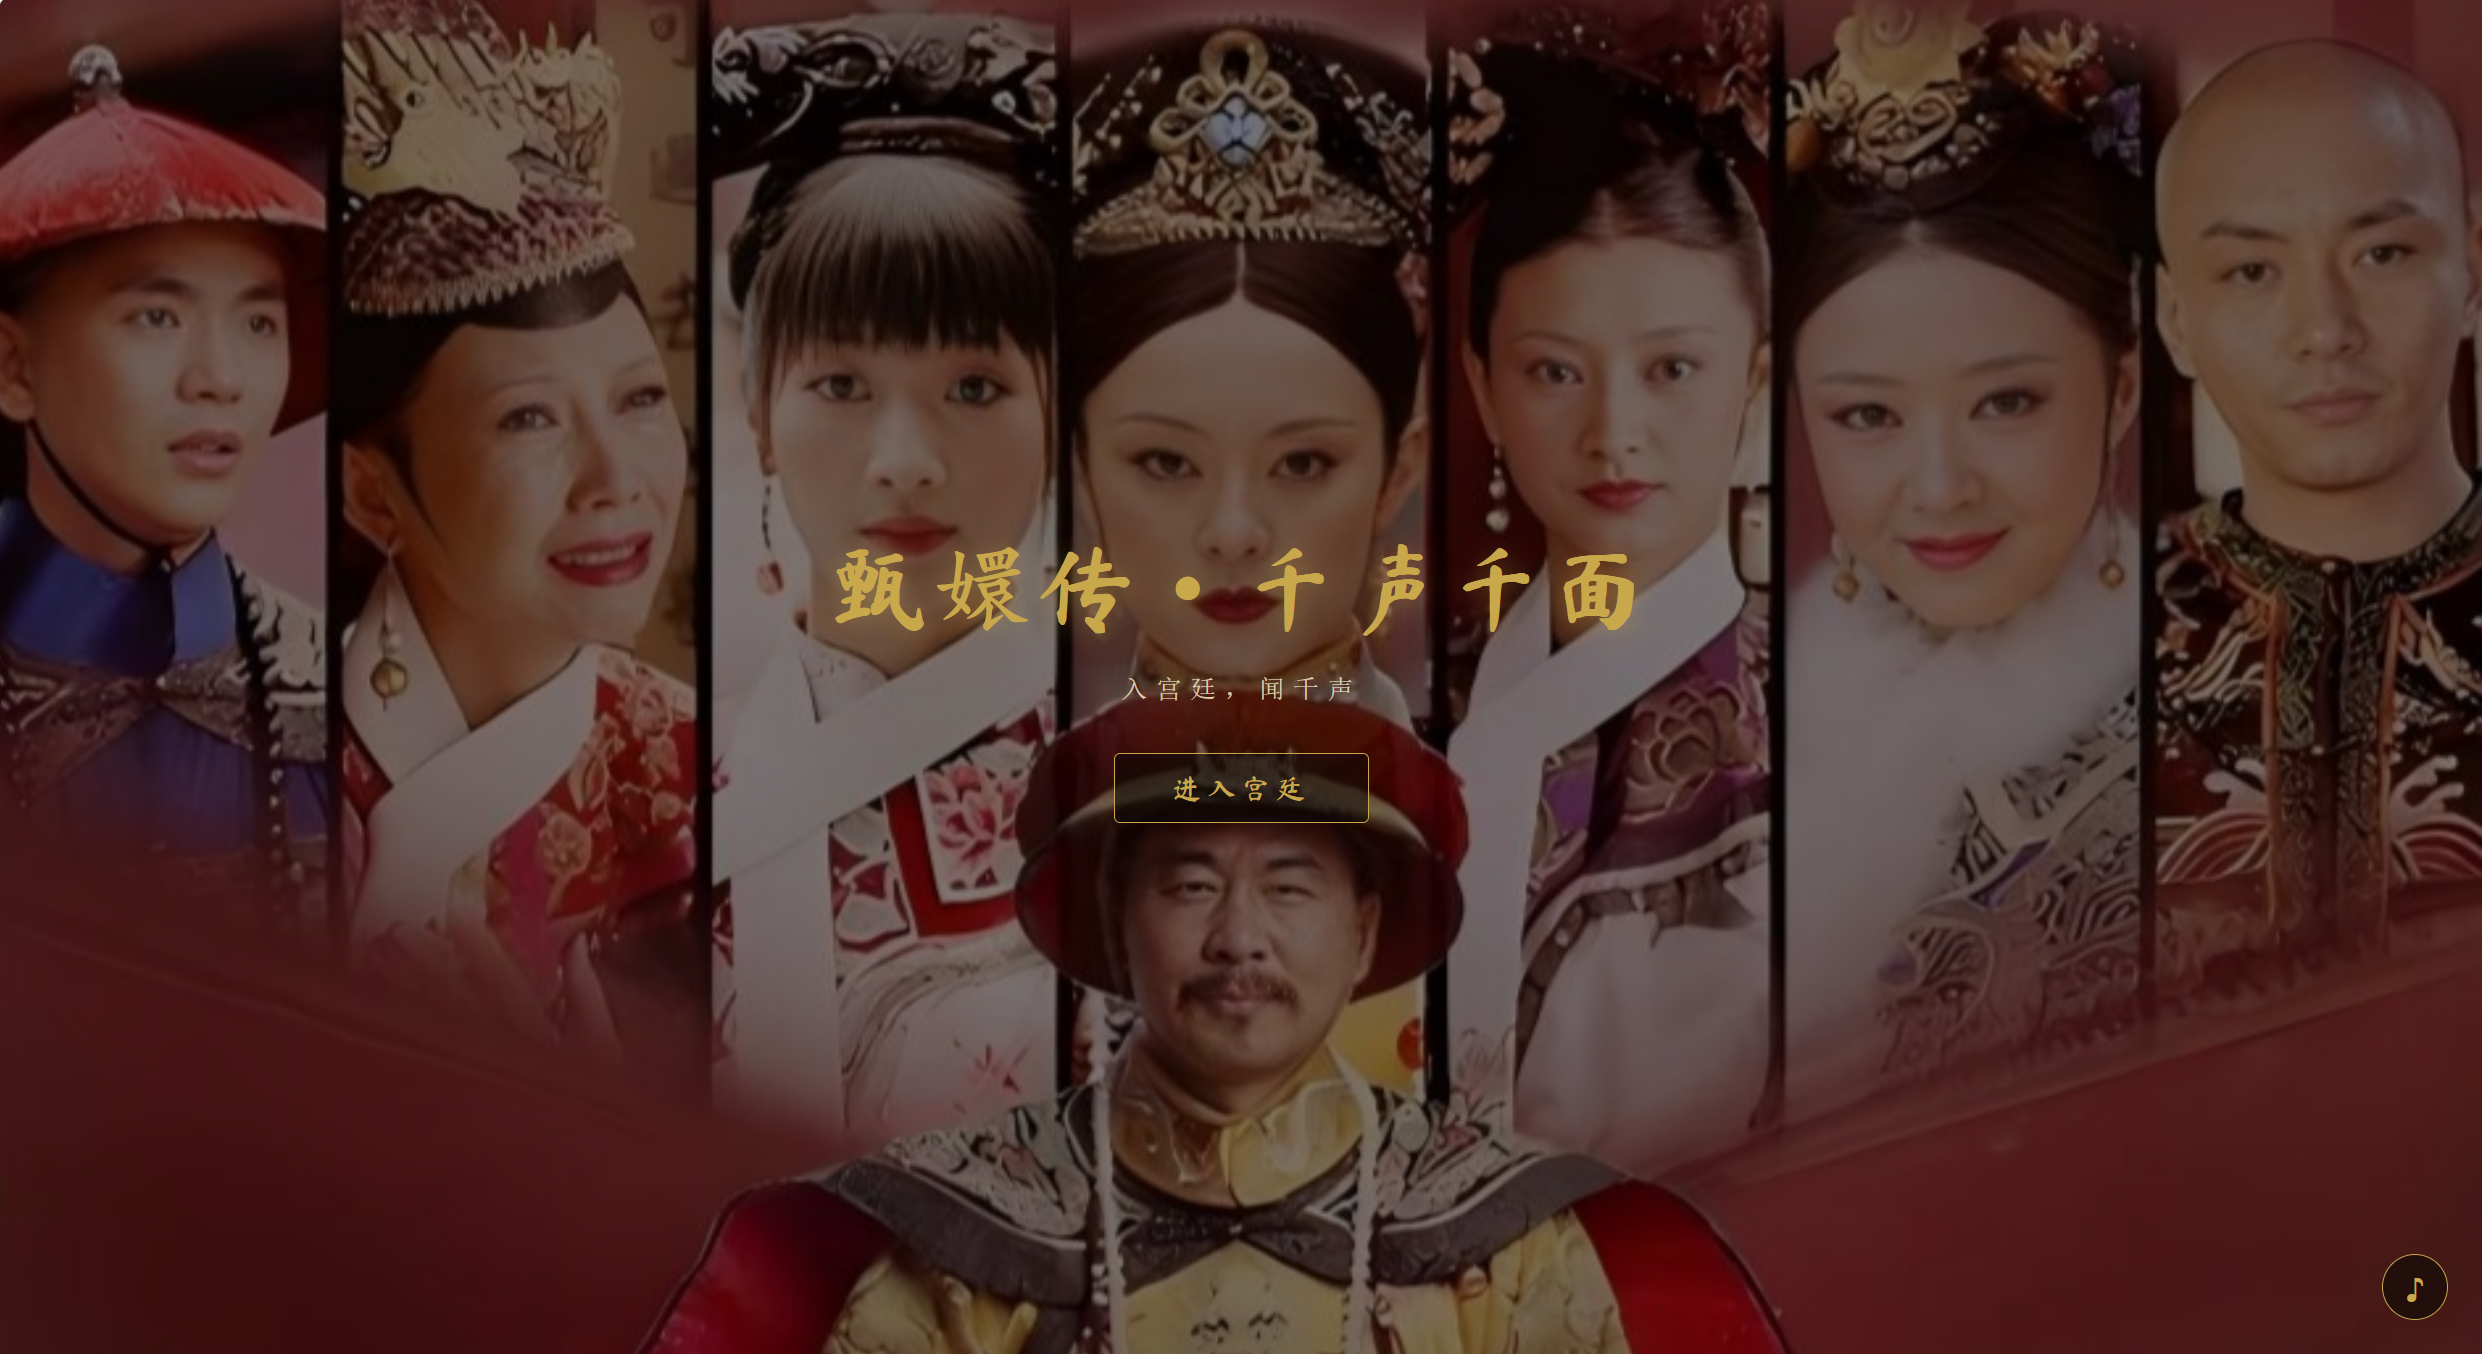
\includegraphics[width=0.85\textwidth]{figures/ui_homepage.png}
\caption{系统主页界面}
\label{fig:ui-home}
\end{figure}

\paragraph{角色选择页（CharacterSelectPage）}
提供三种交互模式入口：\textbf{现代来客}（以现代人身份入宫对话）、\textbf{宫廷中人}（扮演剧中角色参与对话）和\textbf{即兴对话}（选择两个 AI 角色自动对戏）。选择身份后展示 14 张角色卡片，每张包含角色剧照、角色名（毛笔体）和一句经典台词。卡片具有悬停放大与金色边框高亮效果。三种模式的选择界面分别如图~\ref{fig:ui-select-modern}、图~\ref{fig:ui-select-palace}和图~\ref{fig:ui-select-duet}所示。

\begin{figure}[H]
\centering
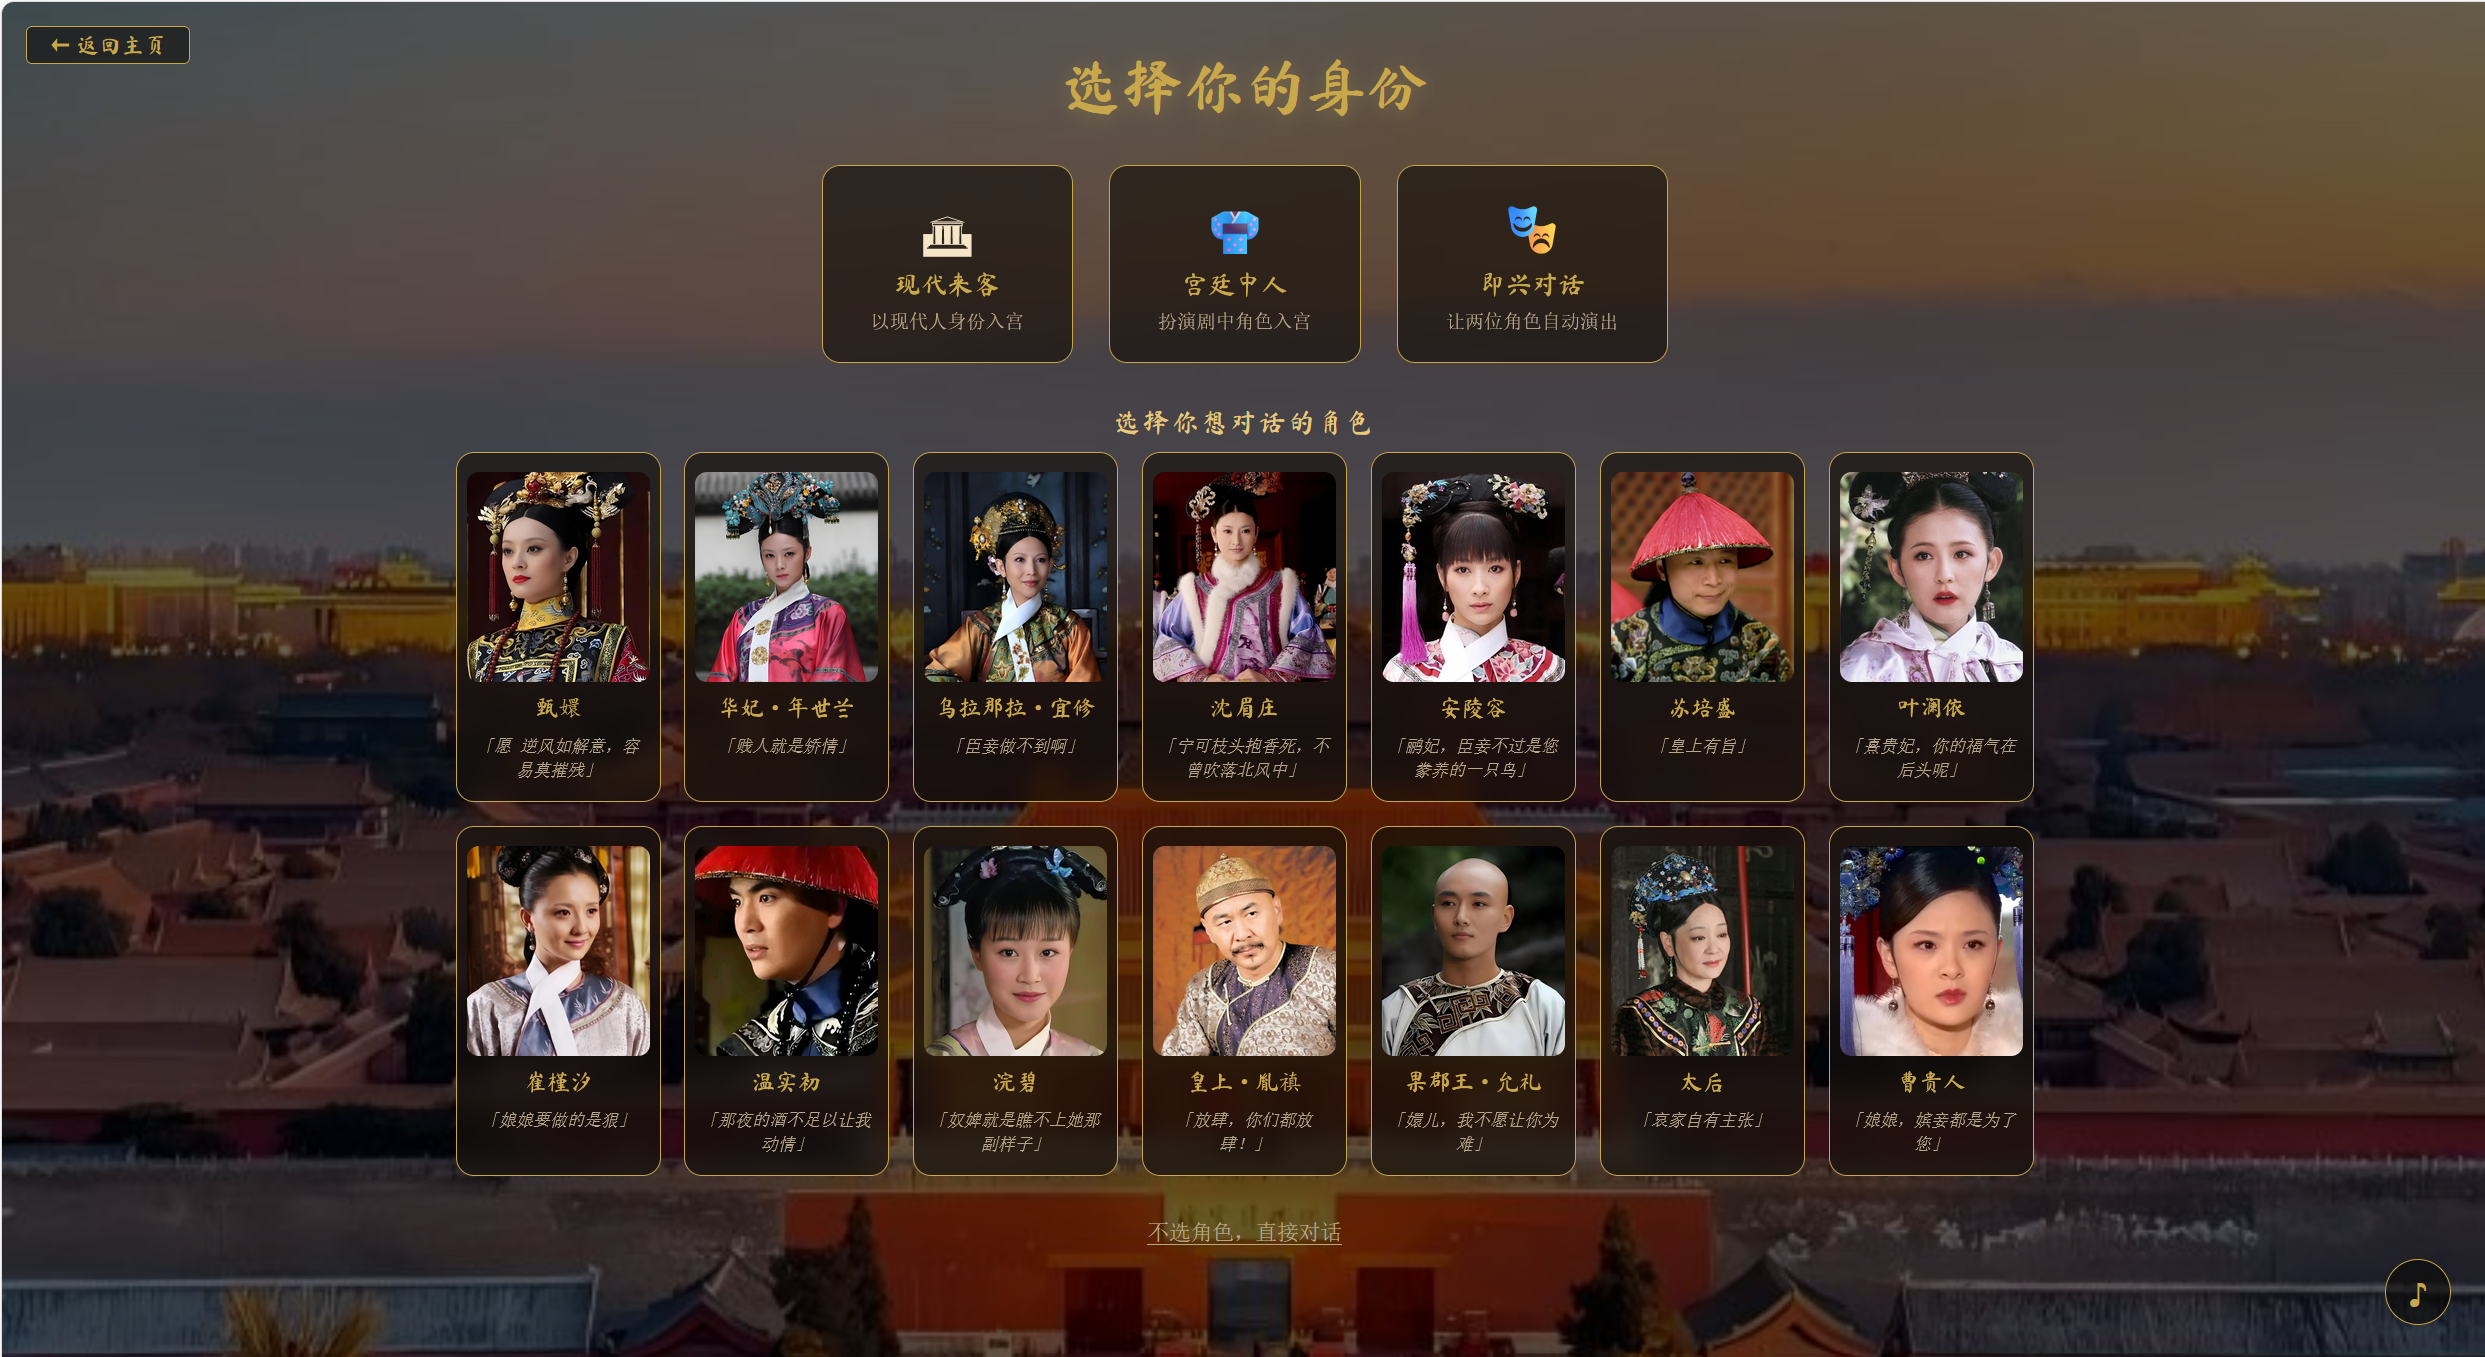
\includegraphics[width=0.85\textwidth]{figures/ui_select_modern.png}
\caption{角色选择页------现代来客模式}
\label{fig:ui-select-modern}
\end{figure}

\begin{figure}[H]
\centering
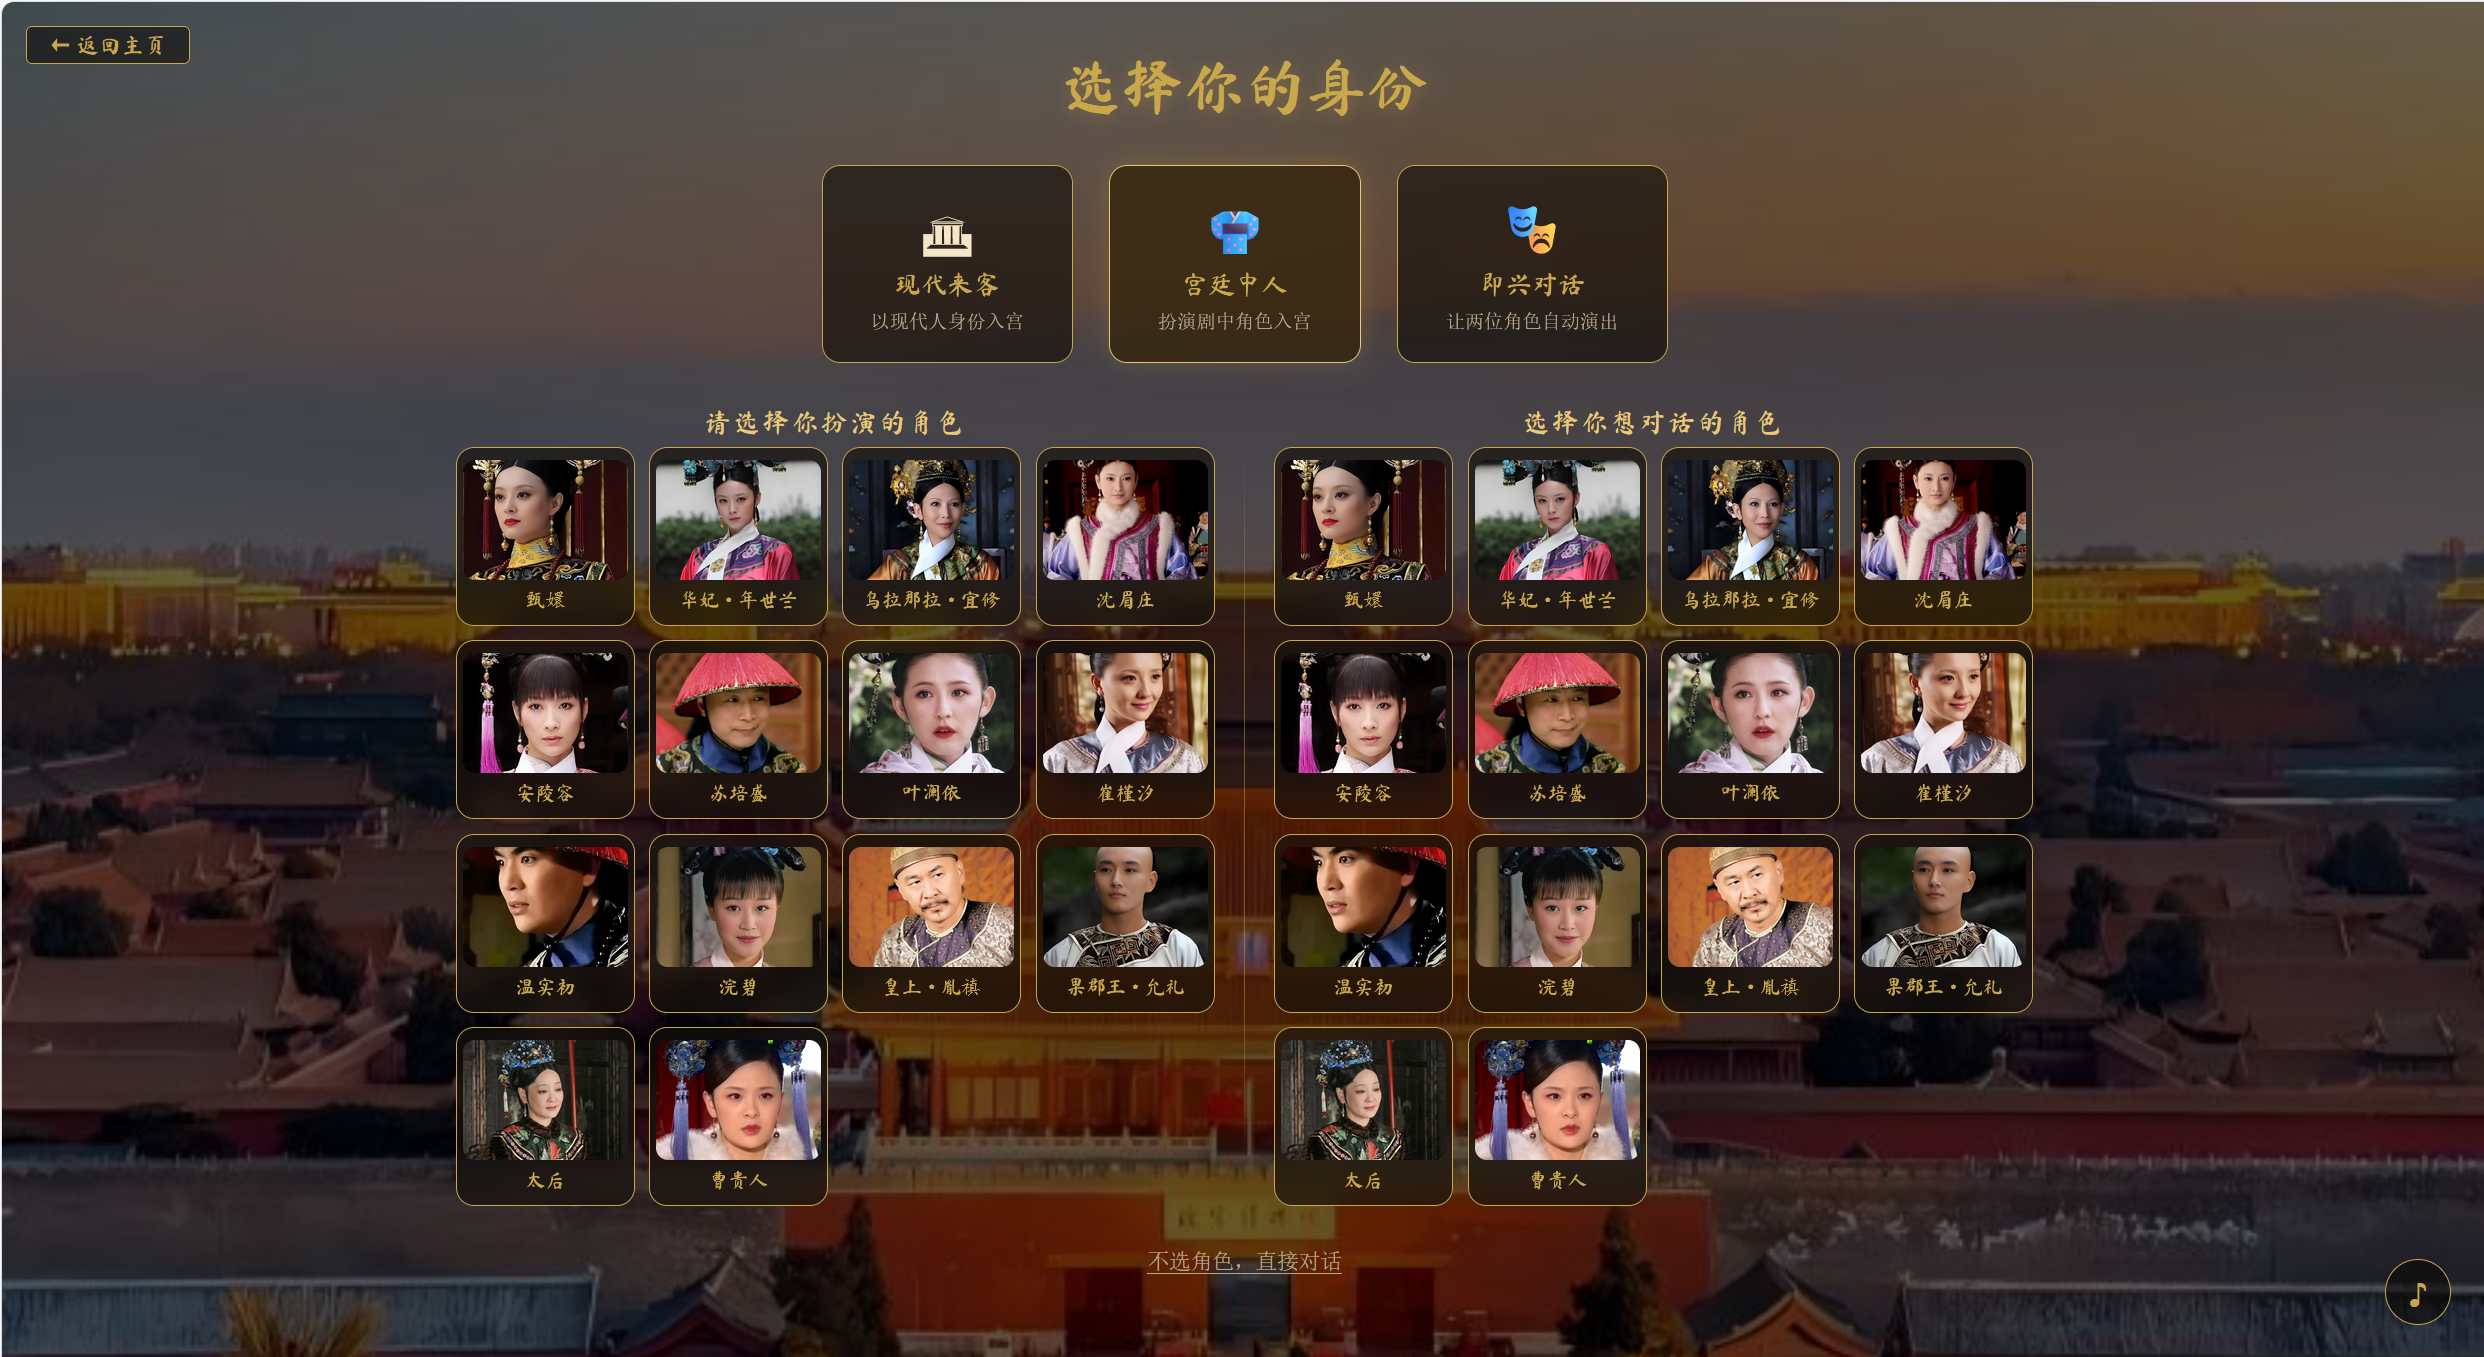
\includegraphics[width=0.85\textwidth]{figures/ui_select_palace.png}
\caption{角色选择页------宫廷中人模式（左：选择扮演角色，右：选择对话角色）}
\label{fig:ui-select-palace}
\end{figure}

\begin{figure}[H]
\centering
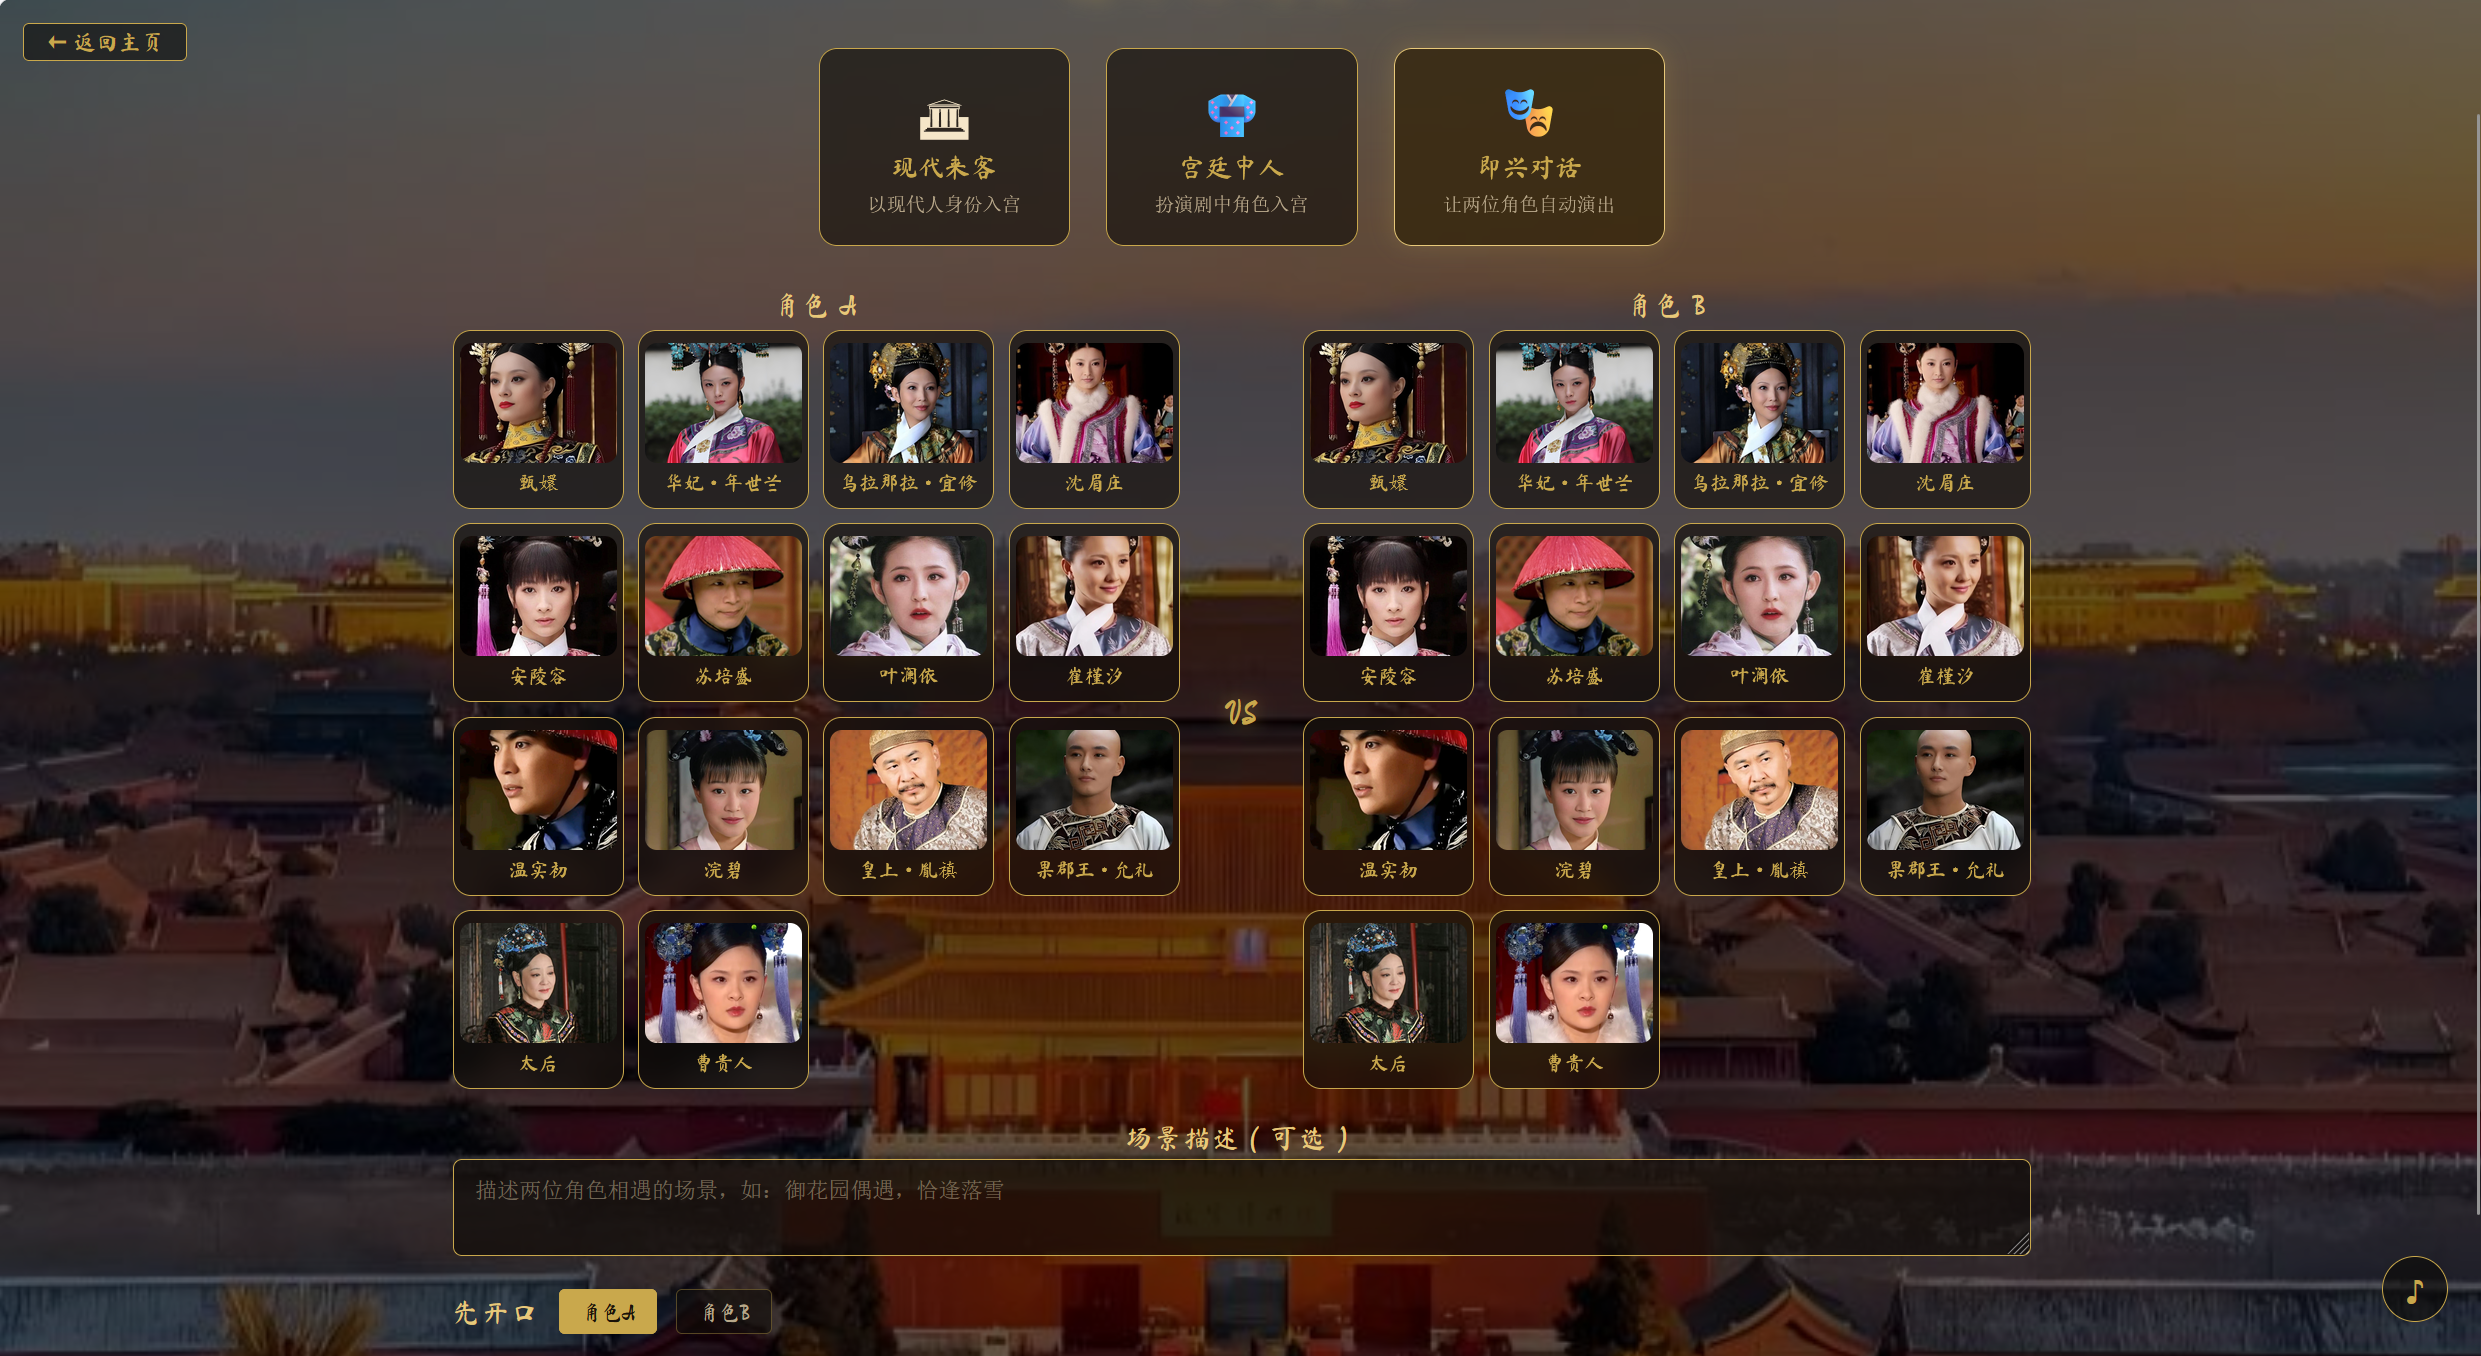
\includegraphics[width=0.85\textwidth]{figures/ui_select_duet.png}
\caption{角色选择页------即兴对话模式（左右各选一位角色 + 场景描述）}
\label{fig:ui-select-duet}
\end{figure}

\paragraph{对话页（ChatPage）}
采用左右两侧角色展示区 + 中间对话区的三栏布局（比例约 1:3:1）。两侧角色展示区显示当前角色剧照与声波动画，背景图根据对话角色动态切换。中间对话区支持文字输入、语音输入（浏览器 MediaRecorder API 录音 $\to$ ASR 识别 $\to$ 回填输入框）、快捷经典台词按钮、TTS 引擎实时切换（GPT-SoVITS / CosyVoice）和情绪手动覆盖。LLM 返回的情绪标签会触发对应视觉反馈：愤怒时背景闪烁红色遮罩，悲伤时亮度降低，喜悦时出现金色光晕。

% TODO: 补充单人对话截图
% \begin{figure}[H]
% \centering
% 
\includegraphics[width=0.85\textwidth]{figures/ui_chat.png}
% \caption{单人智能对话界面}
% \label{fig:ui-chat}
% \end{figure}

点击结束对话后弹出总结卡片，包含角色态度评价和古风总结语，支持通过 html2canvas 一键导出 PNG。

% TODO: 补充对话总结截图
% \begin{figure}[H]
% \centering
% 
\includegraphics[width=0.5\textwidth]{figures/ui_summary.png}
% \caption{对话总结卡片}
% \label{fig:ui-summary}
% \end{figure}

\paragraph{即兴对话页（DuetPage）}
用户选择两个角色并设定场景后，两个 AI 角色自动交替对话，用户全程旁观。后端循环调用 LLM 生成回复并通过 SSE 逐轮推送文本与合成音频，前端使用 Web Audio API 按序排队播放，形成即兴对戏效果。用户可随时点击停止按钮中断对话。

% TODO: 补充双人即兴对话截图
% \begin{figure}[H]
% \centering
% 
\includegraphics[width=0.85\textwidth]{figures/ui_duet.png}
% \caption{双人即兴对话界面}
% \label{fig:ui-duet}
% \end{figure}

\subsubsection{流式 TTS 链路}

CosyVoice 引擎支持流式语音合成，系统实现了完整的 SSE 流式播放链路，如图~\ref{fig:stream-tts}所示。

\begin{figure}[H]
\centering
\begin{tikzpicture}[node distance=1.6cm, auto, scale=0.82, every node/.style={transform shape}]

    \node [cterm, minimum width=5.0cm]
        (tts) {\textbf{CosyVoice TTS 服务} (\texttt{:8003}) \\ {\footnotesize AutoDL 云端，流式生成音频块}};
    \node [cproc, below=1.6cm of tts, minimum width=5.0cm]
        (mid) {\textbf{yiping-backend} (\texttt{:8000}) \\ {\footnotesize SSE 转发，每块 \texttt{\{i, audio, dur\}}}};
    \node [cproc, below=1.6cm of mid, minimum width=5.0cm]
        (web) {\textbf{前端 Web Audio API} \\ {\footnotesize 按序号 \texttt{i} 计算 startTime 排队}};
    \node [cterm, below=1.6cm of web, minimum width=5.0cm]
        (play) {\textbf{无缝顺序播放} \\ {\footnotesize 首音延迟 $\sim$1.5s，RTF 0.5\textasciitilde 0.8}};

    \draw [carr] (tts) -- node[right, font=\scriptsize\color{Cdark}, xshift=2pt]{SSH 隧道} (mid);
    \draw [carr] (mid) -- node[right, font=\scriptsize\color{Cdark}, xshift=2pt]{SSE 推送} (web);
    \draw [carr] (web) -- node[right, font=\scriptsize\color{Cdark}, xshift=2pt]{AudioContext 调度} (play);

\end{tikzpicture}
\caption{CosyVoice 流式 TTS 播放链路}
\label{fig:stream-tts}
\end{figure}

流式方案相比非流式方案将首音延迟从 2\textasciitilde 3 秒降低至约 1.5 秒，音频块到达后立即解码并按序号计算播放起始时间，即使网络导致块乱序也能保证播放顺序正确。

% ══════════════════════════════════════════════════════════════════════════
\section{实验结果}
\label{sec:results}

% ── 4.1 数据集构建结果 ────────────────────────────────────────────────────
\subsection{数据集构建结果}
\label{sec:result-data}

% [成员A负责撰写]
% 此部分展示数据集构建的最终成果，包括：
%
% 1. 14角色数据分布表（角色名、片段数、时长、占比）
% 2. 数据清洗各步骤的过滤效果统计
% 3. 聚类效果分析（KMeans准确率, 淘汰原因）
%
% 建议配合数据分布柱状图或饼图

\subsection{语音合成效果对比}
\label{sec:result-tts}

% [成员A+B共同撰写]
% 此部分展示两种TTS引擎的合成效果对比，包括：
%
% 1. CosyVoice3 Zero-shot vs GPT-SoVITS 微调的主观听感对比
% 2. 不同角色的音色还原度评估
% 3. 情绪Speaker方案的效果验证
% 4. 流式 vs 非流式TTS的延迟对比（首音延迟、RTF）
%
% 建议配合MOS评分表（如有）或主观评价表

\subsection{对话系统功能验证}
\label{sec:result-dialogue}

% [全组共同撰写]
% 此部分展示系统各功能模块的运行效果，包括：
%
% 1. 单人对话效果截图与分析
% 2. 双人即兴对话效果截图与分析
% 3. ASR识别准确率测试
% 4. 情绪视觉反馈与对话总结卡片展示
%
% 建议配合系统运行截图

% ══════════════════════════════════════════════════════════════════════════
\section{问题分析}
\label{sec:problems}

在项目实施过程中，团队遇到并解决了以下关键问题：

\subsection{CosyVoice3 微调过拟合}
\label{sec:prob-overfit}

% [成员A负责撰写]
% 分析内容：
% - 14角色联合微调时，数据极度不均衡（甄嬛占30%，温实初仅2%）导致严重过拟合
% - Epoch 3开始CV Loss反转上升（3.59→4.59），训练损失持续下降但验证表现恶化
% - 解决方案：果断转向Zero-shot方案，利用预训练模型的泛化能力
% - 经验教训：小规模不均衡数据集不适合端到端微调，Zero-shot是更优选择

\subsection{GPT-SoVITS 训练与调优}
\label{sec:prob-gptsovits}

% [成员B负责撰写]
% 分析内容：
% - 小角色（如温实初仅20分钟数据）微调效果不稳定
% - v4与v2ProPlus版本在不同角色上表现不一，需逐角色选择最优版本
% - LoRA rank选择对过拟合-欠拟合的影响
% - 解决方案：单角色独立微调 + 双版本并行 + LoRA约束

\subsection{情绪控制与音色保真的矛盾}
\label{sec:prob-emotion}

% [成员A负责撰写]
% 分析内容：
% - Zero-shot可完美复现中性音色，但无法自然表达情绪
% - Instruct方式控制情绪会导致音色损失
% - 解决方案：情绪Speaker方案——手工采集真实情绪音频注册为独立Speaker
% - 效果：用真实情绪替代指令控制，音色完全不丢失


% ══════════════════════════════════════════════════════════════════════════
\section{总结与展望}
\label{sec:conclusion}

\subsection{项目成果}

本项目成功构建了《甄嬛传》多角色语音对话系统，主要成果如下：

\begin{itemize}[leftmargin=*]
    \item 自主构建了包含 14 个角色、13,605 段语音片段、总时长约 16.7 小时的高质量中文语音数据集。
    \item 实现了 CosyVoice3 Zero-shot（30 个 Speaker）与 GPT-SoVITS 微调（28 组权重）的双引擎语音合成。
    \item 创新性地提出了\textbf{情绪 Speaker}方案，通过 107 段手工采集的真实情绪音频实现了 4 种情感语音合成，有效解决了情绪控制与音色保真的矛盾。
    \item 实现了单人智能对话与双人即兴对戏两种交互模式，支持流式语音播放，首音延迟约 1.5 秒。
    \item 构建了完整的前后端系统，包含古风宫廷风格 UI、FastAPI 中间层和云端 GPU 服务。
\end{itemize}

\subsection{未来展望}

\begin{itemize}[leftmargin=*]
    \item 扩充更多角色（如端妃、敬妃、流朱等）和更多情绪类别。
    \item 探索更高效的微调策略（如单角色独立微调 + LoRA），解决数据不均衡下的过拟合问题。
    \item 引入数字人技术（SadTalker / MuseTalk），在算力允许时实现角色视频对话。
\end{itemize}

% ══════════════════════════════════════════════════════════════════════════
% 参考文献（后续在正文中用到时再逐条添加）
% ══════════════════════════════════════════════════════════════════════════
\newpage
\phantomsection
\addcontentsline{toc}{section}{参考文献}

\begin{thebibliography}{99}

% TODO: 在正文中需要引用时，在此添加对应条目并在正文处标注 \cite{key}
% 预留常用条目（取消注释并在正文中引用即可）：
%
% \bibitem{wang2023valle} Wang C, Chen S, Wu Y, et al. Neural Codec Language Models are Zero-Shot Text to Speech Synthesizers[C]. arXiv:2301.02111, 2023.
% \bibitem{du2024cosyvoice} Du Z, Chen S, Ma Z, et al. CosyVoice 2: Scalable Streaming Speech Synthesis with Large Language Models[C]. arXiv:2412.10117, 2024.
% \bibitem{gptsovits} RVC-Boss. GPT-SoVITS[EB/OL]. https://github.com/RVC-Boss/GPT-SoVITS, 2024.
% \bibitem{whisper} Radford A, Kim J W, Xu T, et al. Robust Speech Recognition via Large-Scale Weak Supervision[C]. ICML, 2023.
% \bibitem{funasr} Gao Z, Li Z, Wang J, et al. FunASR: A Fundamental End-to-End Speech Recognition Toolkit[C]. Interspeech, 2023.
% \bibitem{uvr5} Anjok07. Ultimate Vocal Remover GUI v5[EB/OL]. https://github.com/Anjok07/ultimatevocalremovergui, 2023.
% \bibitem{3d-speaker} Chen Z, Yao Y, Zheng S, et al. 3D-Speaker[C]. arXiv:2306.15354, 2023.
% \bibitem{faster-whisper} SYSTRAN. faster-whisper[EB/OL]. https://github.com/SYSTRAN/faster-whisper, 2023.

\end{thebibliography}

% ══════════════════════════════════════════════════════════════════════════
% 小组成员分工
% ══════════════════════════════════════════════════════════════════════════
\newpage
\phantomsection
\addcontentsline{toc}{section}{小组成员分工}
\section*{小组成员分工}

\begin{table}[H]
\centering
\renewcommand{\arraystretch}{1.5}
\begin{tabularx}{\textwidth}{p{2.0cm}p{2.0cm}p{1.8cm}X}
\toprule
\textbf{成员} & \textbf{姓名} & \textbf{学号} & \textbf{负责内容} \\
\midrule
成员A & 李思婷 & 2023212061 &
\begin{minipage}[t]{\linewidth}
\begin{itemize}[leftmargin=*, nosep, topsep=0pt]
    \item 数据集构建：76集原剧音频处理全流程（人声分离→VAD切分→ASR转写→声纹聚类→人工标注→数据清洗）
    \item CosyVoice3-0.5B 微调实验与过拟合分析
    \item CosyVoice3 Zero-shot 方案：14角色Speaker注册
    \item 情绪Speaker创新方案：手工采集107段真实情绪音频，注册16个情绪Speaker
\end{itemize}
\end{minipage} \\
\midrule
成员B & 张笑 & 2023212062 &
\begin{minipage}[t]{\linewidth}
\begin{itemize}[leftmargin=*, nosep, topsep=0pt]
    \item GPT-SoVITS 微调：14角色$\times$2版本=28组独立权重训练
    \item ASR 模块：faster-whisper-small 部署与配置
    \item LLM 对话模块：角色人设Prompt设计、单人对话与双人即兴对话生成
    \item GPT-SoVITS 服务端部署与情绪参考音频路由
    \item 参与情绪音频采集与标注
\end{itemize}
\end{minipage} \\
\midrule
成员C & 黄艺平 & 2023212179 &
\begin{minipage}[t]{\linewidth}
\begin{itemize}[leftmargin=*, nosep, topsep=0pt]
    \item 前端设计：React古风宫廷UI（主页、角色选择、对话、即兴对话四页面）
    \item 视觉素材采集：12张角色剧照、11张场景背景图、1首背景音乐
    \item yiping-backend 中间层：统一API网关、云端服务路由与对接
    \item 流式TTS链路集成：SSE + Web Audio API 排队播放
\end{itemize}
\end{minipage} \\
\bottomrule
\end{tabularx}
\caption{小组成员分工详情}
\label{tab:team}
\end{table}

\end{document}
